\section{DEB}

\newcommand{\ddir}{"\texttt{debian}" directory}
\newcommand{\dpkg}{"\bftt{dpkg}" command}

The next pages will focus on building a DEB ("\texttt{.deb}") file suitable for distribution by \href{https://www.debian.org}{Debian} Linux. \\[0.25cm]
Maybe more importantly I will assume that you are working on Debian Linux, that would make
a lost of sense since we are talking about building Debian DEBs here. Some of the commands
I will use thereafter can only be found on Debian based Linux, therefore I would recommend to download
and install the latest Debian version either on your computer or in a virtual machine. \\[0.25cm]
To prepare a DEB file you need first to install the appropriate tools:
{\small{
\begin{script}
\uprompt{~} sudo apt install build-essential dh-make devscripts 
\uprompt{~} sudo apt install debhelper sbuild schroot debootstrap
\uprompt{~} sudo apt install debmake debmake-doc reportbug 
\uprompt{~} sudo apt install piuparts piuparts-master piuparts-slave
\end{script}
}}
\\[-0.25cm]
\noindent \bftt{dpkg} (for \bftt{D}ebian \bftt{p}ac\bftt{k}a\bftt{g}e) is the tool managing package distribution on Debian based Linux distributions. 
If I intend to provide tips and trick to help you prepare your DEB, I strongly recommend that you give a look to:
\begin{itemize}
\item \href{https://wiki.debian.org/Packaging/Intro?action=show\&redirect=IntroDebianPackaging}{Introduction to Debian Packaging}
\item \href{https://wiki.debian.org/HowToPackageForDebian}{How to package for Debian}
\item \href{https://www.debian.org/doc/debian-policy/}{Debian policy}
\item \href{https://www.debian.org/doc/manuals/packaging-tutorial/packaging-tutorial.fr.pdf}{Tutoriel: la construction de paquets Debian}
\item \href{https://wiki.debian.org/SimplePackagingTutorial}{Simple packaging tutorial}
\item \href{file://usr/share/doc/debmake-doc/}{debmake documentation}
\end{itemize}
Indeed this guide is not meant to be a thorough review of DEB packaging, that is actually
much more complicated than for the simple desktop application used afterward to illustrate the process.

\newpage
\subsection{Prerequisites}
\label{dprereq}
We will briefly introduce hereafter the basics of Debian package construction. \\
Before starting few considerations are in order:
\begin{itemize}
\item It is required to setup properly some information and aliases.\\
To do that edit the "\texttt{\textasciitilde/.bashrc}" file and add the following lines:
\begin{scripti}
\comm{Debian packager identification}
\bad{export} \dctt{DEBEMAIL}\bad{=}\reg{\email}
\bad{export} \dctt{DEBFULLNAME}\bad{=}\reg{Your Name}

\comm{Improved lintian command for package verification}
\bad{alias} \dctt{lintian}\bad{=}\reg{lintian -EviIL +pedantic --color auto}
\end{scripti}
\item For Debian packaging to be successful the folder with the sources \red{\bf{\textsc{must}}} be of the form: 
\begin{scripti}name-version\end{scripti}
\\[-0.75cm]
With: 
\begin{itemize}
\item \texttt{name}: the package name, in example afterwards: "\texttt{program}"
\item \texttt{version}: the version number(s), in example afterwards: "\texttt{1.2.12}"
\end{itemize}
\vspace{-1cm}
\begin{scripti}
\uprompt{~} mkdir program-1.2.12
\uprompt{~} cd program-1.2.12
\end{scripti}
\\[-0.75cm]
\noindent And copy the sources in this directory. 
\end{itemize}
The process of preparing a Debian package for your program is called "Debianization", 
so let's go and Debianize away !

\newpage
\subsection{The \ddir}

The Debian package will be built using information in the \ddir\ that must be located with your sources:
{\footnotesize{
\begin{script}
\uprompt{~/program-1.2.12} ls -lh
-rw-r--r--.  1 user group  54K 24 mars  17:28 aclocal.m4
-rw-r--r--.  1 user group  481 24 mars  11:24 AUTHORS
drwxr-xr-x.  2 user group 4,0K 24 mars  17:28 \btt{autom4te.cache}
-rw-r--r--.  1 user group 2,8K 24 mars  11:24 ChangeLog
lrwxrwxrwx.  1 user group   32 24 mars  17:24 \gtt{compile}
lrwxrwxrwx.  1 user group   37 24 mars  17:24 \gtt{config.guess}
lrwxrwxrwx.  1 user group   35 24 mars  17:24 \gtt{config.sub}
-rwxr-xr-x.  1 user group 243K 24 mars  17:28 \gtt{configure}
drwxr-xr-x   5 user group 4,0K 19 sept. 17:20 \rtt{debian}
-rw-r--r--.  1 user group 3,6K 24 mars  11:24 configure.ac
-rw-r--r--.  1 user group  34K 24 mars  11:24 COPYING
drwxr-xr-x.  2 user group 4,0K 24 mars  11:24 \btt{data}
lrwxrwxrwx.  1 user group   32 24 mars  17:24 \gtt{depcomp}
-rw-r--r--.  1 user group  34K 24 mars  11:24 config.h.in
-rw-r--r--.  1 user group  16K 24 mars  11:24 INSTALL
lrwxrwxrwx.  1 user group   35 24 mars  17:24 \gtt{install-sh}
-rw-r--r--.  1 user group 4,0K 24 mars  17:03 Makefile.am
drwxr-xr-x.  2 user group 4,0K 24 mars  11:24 \btt{metadata}
lrwxrwxrwx.  1 user group   32 24 mars  17:24 \gtt{missing}
-rw-r--r--.  1 user group  247 24 mars  11:24 NEWS
drwxr-xr-x.  4 user group 4,0K 24 mars  11:24 \btt{pixmaps}
-rw-r--r--.  1 user group 4,8K 24 mars  11:24 README
drwxr-xr-x.  2 user group 4,0K 24 mars  11:24 \btt{src}
\end{script}
}}
\noindent You can generate a ready to use "\rtt{debian}" directory using:
{\footnotesize{
\begin{script}
\uprompt{~/program-1.2.12} \bftt{debmake}
\end{script}
}}
\\[-0.5cm]
\noindent If no \ddir\ is present then this command will create it, including sample files to work on. 
However this sample \ddir\ will contain some files likely unnecessary to build your first simple Debian package. \\[0.25cm]
I recommend to start working with the following files and directories:
{\footnotesize{
\begin{script}
\uprompt{~/program-1.2.12} ls -lh debian
-rw-r--r-- 1 user group  586 19 sept. 17:22 changelog
-rw-r--r-- 1 user group 3,2K 19 sept. 17:22 control
-rw-r--r-- 1 user group  39K 19 sept. 17:22 copyright
drwxr-xr-x 1 user group 4,0K 19 sept. 17:22 \btt{patches}
-rw-r--r-- 1 user group  137 19 sept. 17:22 program.install
-rw-r--r-- 1 user group   46 19 sept. 17:22 program-data.install
-rwxr-xr-x 1 user group  103 19 sept. 17:22 \gtt{rules}
drwxr-xr-x 2 user group 4,0K 19 sept. 17:22 \btt{source}
drwxr-xr-x 2 user group 4,0K 19 sept. 17:22 \btt{upstream}
-rw-r--r-- 1 user group  183 19 sept. 17:22 watch
\end{script}
}}
\\
\noindent Note that the files "\texttt{program.install}" and "\texttt{program-data.install}" are not created by the \bftt{debmake} command.  
%\begin{itemize}
%\item \bftt{patches}
%{\footnotesize{
%\begin{scripti}
%\uprompt{~/program-1.2.12} ls -lh debian/patches
%
%\end{scripti}
%}}
%\item \bftt{source}
%{\footnotesize{
%\begin{scripti}
%\uprompt{~/program-1.2.12} ls -lh debian/source
%
%\end{scripti}
%}}
%\item \bftt{upstream}
%{\footnotesize{
%\begin{scripti}
%\uprompt{~/program-1.2.12} ls -lh debian/upstream
%
%\end{scripti}
%}}
%\end{itemize}
\subsubsection{The "\texttt{changelog}" file}

The "\texttt{changelog}" file is to be updated for each new release of the program or the package, 
it describes briefly the changes in the new version:
\begin{script}
\uprompt{~/program-1.2.12} cat debian/changelog
program (1.2.12-2) unstable; urgency=medium

  * New package version

 -- Your Name <\email>  Tue, 19 Sep 2023 15:45:00 +0200

program (1.2.12-1) unstable; urgency=medium

  * Bug corrections and improvements.
  * See: \gitprog/releases/tag/v1.2.12

 -- Your Name <\email>  Mon, 17 Jul 2023 17:26:00 +0200
\end{script}

\subsubsection{The "\texttt{control}" file}

The "\texttt{control}" file contains build and runtime dependencies for your program. \\
To prepare this file requires to find the appropriate package name for each dependencies of your program: 
\begin{itemize}
\item For building the program: in the section "\texttt{Build-Depends}"
\item For running the program: in the section(s) "\texttt{Depends}" 
\end{itemize}
Dependencies are presented using coma separated lists, parenthesis can be used for specific requirement. \\
Note that the following example illustrates a "\texttt{control}" file with 2 "\texttt{Package:}" instructions, therefore 2 packages will be created:
\begin{itemize}
\item A package, architecture dependent, for the binary: "\texttt{Package: program}"
\item A package for all non-architecture dependent data: "\texttt{Package: program-data}" 
\end{itemize}
This is a standard way of doing things in the Debian world. \\
{\footnotesize{
\begin{script}
\uprompt{~/program-1.2.12} vi debian/control
\bad{Source:} program
\bad{Section:} science
\bad{Priority:} optional
\bad{Maintainer:} \var{Your Name <\email>}
\bad{Uploaders:} \var{Your Name <\email>}
\bad{Build-Depends:} debhelper-compat (= 13),
                  automake,
                  autoconf,
                  pkg-config,
                  gfortran,
                  libgfortran5,
                  libgtk-3-dev,
                  libxml2-dev,
                  libpango1.0-dev,
                  libglu1-mesa-dev,
                  libepoxy-dev,
                  libavutil-dev,
                  libavcodec-dev,
                  libavformat-dev,
                  libswscale-dev,
                  desktop-file-utils,
                  appstream-util
\bad{Standards-Version:} 4.6.2
\bad{Homepage:} \var{https://www.prog.com}
\bad{Vcs-Browser:} \var{\gitprog}
\bad{Vcs-Git:} \var{\gitprog.git}
\bad{Rules-Requires-Root:} no

\bad{Package:} program
\bad{Architecture:} any
	\bad{Depends:} program-data (= \var{\$\{source:Version\}}),
          \var{\$\{shlibs:Depends\}}, \var{\$\{misc:Depends\}},
          libgtk-3-0,
          libglu1-mesa,
          bash-completion
\bad{Description:} program is doing something
 Program is a tool box to analyze many things
 .
 This package provides the binaries.

\bad{Package:} program-data
\bad{Architecture:} all
\bad{Multi-Arch:} foreign
\bad{Depends:} \var{\$\{misc:Depends\}}
\bad{Enhances:} program
\bad{Suggests:} program
\bad{Description:} program is doing something (data)
 Program is a tool box to analyze many things
 .
 This package contains data files for program.
\end{script}
}}
\newpage
\noindent Few tips to help you prepare this file:
\begin{itemize}
\item The "\texttt{Section:}" keyword allows to select where the program will appear in the applications menu
\item The value for "\texttt{Standards-Version:}" changes with the Debian version:
\begin{itemize} 
\item For Debian 11: \texttt{4.5.1}
\item For Debian 12: \texttt{4.6.2}
\end{itemize}
\item The short description follows the instruction "\texttt{Description}" on the same line
\item The long description start on the next line: 
\begin{itemize}
\item Every line of the long description must start by a space character
\item Every blank line is specified using a space followed by a dot character: "\texttt{ .}"
\end{itemize}
\end{itemize}

\subsubsection{The "\texttt{copyright}" file}

The "\texttt{copyright}" file is likely the most complicated file to prepare for Debian packaging. \\
This file describes the licensing of every file in your package: 
\begin{itemize}
\item The software license for your program
\item The software license for every third-party library you ship together with the program
\item The software licence for every file in your source code with specific copyright attribution 
\end{itemize}
In each case license information must includes:
\begin{itemize}
\item The name of the software license
\item A short, if available, otherwise complete text description of the license:
\begin{itemize}
\item Every line of the license text must start by a space character
\item Every blank line in the license text is specified by a space followed by a dot: "\texttt{ .}"
\end{itemize}
\end{itemize}
The first instructions in the "\texttt{copyright}" file are providing contact information, afterwards the "\texttt{copyright}" file is organized as follow, 
with a section listing the files and the associated license:
\begin{script}
\bad{Files:}     file(s) name(s) 
\bad{Copyright:} year(s) copyright owner
\bad{License:}   License-Keyword
\end{script}
Follow later on by the associated license text information:
\begin{script}
\bad{License:} License-Keyword
 Text of the license
\end{script}
\noindent \texttt{License-keyword} information, should use the SPDX identifier: \href{https://spdx.org/licenses/}{https://spdx.org/licenses/} \\[0.5cm]
\noindent Example: 
{\footnotesize{
\begin{script}
\uprompt{~/program-1.2.12} vi debian/copyright
\bad{Format:} https://www.debian.org/doc/packaging-manuals/copyright-format/1.0/
\bad{Upstream-Name:} \var{program}
\bad{Upstream-Contact:} \var{\email}
                     \var{Your Name <\email>}
\bad{Source:} \var{\gitprog/}

\bad{Files:}      *
\bad{Copyright:} 2023-2024 Your Name
\bad{License:}   \bftt{AGPL-3.0-or-later}

\bad{Files:}      Makefile.in
             src/Makefile.in
\bad{Copyright:} 1994-2021 Free Software Foundation, Inc.
\bad{License:}   \bftt{FSFULLR}

\bad{Files:}      aclocal.m4
\bad{Copyright:} 1996-2020 Free Software Foundation, Inc.
             2004 Scott James Remnant <scott@netsplit.com>.
             2012-2015 Dan Nicholson <dbn.lists@gmail.com>
\bad{License:}   \bftt{FSFULLR} and \bftt{GPL-2.0-or-later}
\end{script}
}}
\noindent ... All other files with a license in your package must be listed as well ...
{\footnotesize{
\begin{script}
\bad{Files:}      metadata/com.program.www.appdata.xml
\bad{Copyright:} 2023-2024 Your Name
\bad{License:}   \bftt{FSFAP}

\bad{Files:}      debian/*
\bad{Copyright:} 2023-2024 your Name
\bad{License:}   \bftt{AGPL-3.0-or-later}
\end{script}
}}
\noindent ... Then all license texts are to be inserted after the file list: 
{\footnotesize{
\begin{script}
\bad{License:} \bftt{AGPL-3.0-or-later}
 Text of the AGPL v3.0 or later

\bad{License:} \bftt{FSFULLR}
 Text of the FSULLR

\bad{License:} \bftt{GPL-2.0-or-later}
 Text of the GPL v2.0 or later
\end{script}
}}
A complete example is provided in appendix~\ref{acopy}. 
\newpage
\noindent Note that some tools can be used to help you out in preparing the "\texttt{copyright}" file:
\begin{itemize}
\item \bftt{licensecheck} is command line tool to search licensed file(s) in your sources:
{\footnotesize{
\begin{scripti}
\uprompt{~/program-1.2.12} \bftt{licensecheck} \rtt{-r --copyright} \btt{.}
\end{scripti}
}}
\\[-1.5cm]
\item \bftt{scan-copyrights} helps you create a "\texttt{copyright}" file from scratch:
{\footnotesize{
\begin{scripti}
\uprompt{~/program-1.2.12} \bftt{scan-copyrights}
\end{scripti}
}}
\end{itemize}

\subsubsection{The "\texttt{patches}" directory}

This optional directory contains patch instructions required to build the Debian package, if any. \\
In that case, meaning if source patches are required then the "\texttt{patches}" directory should contain
\begin{itemize}
\item A raw text file named "\texttt{series}" containing the list of all patches to apply. 
\item As many "\texttt{.patch}" files as described in "\texttt{series}", example:
{\footnotesize{
\begin{scripti}
\uprompt{~/program-1.2.12} ls debian/patches
file-1.patch  file-2.patch  series
\uprompt{~/program-1.2.12}
\end{scripti}
}}
\\[-0.5cm]
\noindent With: \\[-0.5cm]
{\footnotesize{
\begin{scripti}
\uprompt{~/program-1.2.12} cat debian/patches/series
file-1.patch
file-2.patch
\uprompt{~/program-1.2.12}
\end{scripti}
}}
\\[-0.5cm]
\noindent And patch file, ex: "\texttt{file-1.patch}", should have the format: \\[-0.5cm] 
{\footnotesize{
\begin{scripti}
\uprompt{~/program-1.2.12} vi debian/patches/file-1.patch
Description: \bftt{this patch is doing this.}  
Author: \bftt{Your Name <\email>}
Forwarded: not-needed
Last-Update: 2023-09-19

\green{--- a/src/file.c
+++ b/src/file.c}
\bbtt{@@ -214,5 +214,5 @@}
   # The next lines to print compilers and flags:
-  printf ("FC    Compiler         : \%s\textbackslash{n}", FC);
\dctt{+  /*printf ("FC    Compiler         : \%s\textbackslash{n}", FC);}
   printf ("FC    Compiler flags   : \%s\textbackslash{n}", FCFLAGS);
   printf ("C     Compiler         : \%s\textbackslash{n}", CC);
-  printf ("C     Compiler flags   : \%s\textbackslash{n}", CFLAGS);
\dctt{+  printf ("C     Compiler flags   : \%s\textbackslash{n}", CFLAGS);*/}
\end{scripti}
}}
\\[-0.75cm] This patch will comment the lines that display compiler flags: when building the package path information is added to the compiler flags 
and you do no want that information to appear in the binary. 
\end{itemize}
To create a patch file use the "\texttt{diff}" command:
{\footnotesize{
\begin{scripti}
\uprompt{~/program-1.2.12} \bftt{diff} \rtt{-u} file.old file.new \bad{>} file.patch
\end{scripti}
}}

\subsubsection{The "\texttt{program.install}" file}

The "\texttt{program.install}" file lists the locations in the system directory tree where files are going to be installed. 
The content of this file depends on the installation process described using in your building system, for the examples listed 
in this manual: 
\begin{script}
\uprompt{~/program-1.2.12} cat debian/program.install
usr/bin
usr/share/applications
usr/share/doc
usr/share/man
usr/share/metainfo
usr/share/mime
usr/share/pixmaps
\end{script}
\noindent For the examples in this manual: \\[0.25cm]
\begin{tabular}{lp{0.25cm}lp{0.25cm}l}
\texttt{usr/bin} & & Executable & & \texttt{prog}\\
\texttt{usr/share/applications} & & Desktop entry & & \texttt{program.desktop} \\
\texttt{usr/share/doc} & & Documentation & & \texttt{README.md} \\
& & & & \texttt{AUTHORS} \\
& & & & \texttt{ChangeLog} \\
\texttt{usr/share/man} & & Manual pages & & \texttt{man1/program.1.gz} \\
\texttt{usr/share/metainfo} & & AppStream metadata & & \texttt{com.program.www.appdata.xml} \\
\texttt{usr/share/mime} & & File association(s) & & \texttt{package/program-mime.xml} \\
\texttt{usr/share/pixmaps} & & Icons and images & & \texttt{program.svg} \\
& & & & \texttt{program-project.svg} \\
& & & & \texttt{program-workspace.svg} \\
\end{tabular}
\noindent You can also have other "\texttt{.install}" file(s):
\begin{script}
\uprompt{~/program-1.2.12} cat debian/program-data.install
usr/share/program
\end{script}
The architecture non-dependent data to be installed with the program, if any.

\subsubsection{The "\texttt{rules}" file}

The \href{https://www.debian.org/doc/debian-policy/ch-source.html#main-building-script-debian-rules}{"\texttt{rules}"} file is an executable makefile 
that contains specific construction rules for your package, keep this file as simple as possible. 
Actually to package a simple application it is unlikely that you will need to modify this file at all. 
{\footnotesize{
\begin{script}
\uprompt{~/program-1.2.12} vi debian/rules
\blue{\#!/usr/bin/make -f}

\comm{Uncomment the next line to enable deb-helper verbose mode} 
\comm{export DH\_VERBOSE = 1}

\bad{export} DEB\_BUILD\_MAINT\_OPTIONS = hardening=+all

\var{\%:}
\qquad\qquad dh \var{\$@}
\end{script}
}}

\subsubsection{The "\texttt{source}" directory}

The \href{https://wiki.debian.org/debian/upstream}{"\texttt{upstream}"}  directory contains a single file: 
{\footnotesize{
\begin{script}
\uprompt{~/program-1.2.12} ls debian/sources
format
\uprompt{~/program-1.2.12} cat debian/sources/format
3.0 (quilt)
\uprompt{~/program-1.2.12}
\end{script}
}}

\subsubsection{The "\texttt{upstream}" directory}

The \href{https://wiki.debian.org/debian/upstream}{"\texttt{upstream}"} directory contains a file in YAML format describing the upstream project being packaged:
{\footnotesize{
\begin{script}
\uprompt{~/program-1.2.12} ls debian/upstream
metadata
\uprompt{~/program-1.2.12} cat debian/upstream/metadata
Bug-Database: \gitprog/issues
Bug-Submit: \gitprog/issues/new
Repository: \gitprog.git
Repository-Browse: \gitprog
Contact: \email
\uprompt{~/program-1.2.12}
\end{script}
}}

\subsubsection{The "\texttt{watch}" file}

\href{https://wiki.debian.org/debian/watch}{"\texttt{watch}"} file is used to check for newer versions of upstream software and to download it if necessary. 
For a GitHub project the syntax is as follow:
{\footnotesize{
\begin{script}
\uprompt{~/program-1.2.12} cat debian/watch
version=4

opts="filenamemangle=s\%(?:.*?)?v?(\textbackslash{d}[\textbackslash{d}.]*)\textbackslash{.}tar\textbackslash{.}gz\%program-\$1.tar.gz\%" \textbackslash
   \gitprog/tags \textbackslash
   (?:.*?/)?v?(\textbackslash{d}[\textbackslash{d}.]*)\textbackslash{.}tar\textbackslash{.}gz debian uupdate
\uprompt{~/program-1.2.12}
\end{script}
}}

\subsection{Building the "\texttt{.deb}" file(s)}

Few recommendations to build the "\texttt{.deb}" file(s): 
\begin{itemize}
\item The commands "\bftt{dh\_make}" and "\bftt{dpkg-buildpackage}" to be used to build the package are sensitive to already existing files in the upper directory, therefore before each build I recommend to clean the working directory:
{\footnotesize{
\begin{scripti}
\uprompt{~} rm -f *\_1.2.12\_*
\uprompt{~} ls
\btt{program-1.2.12}
\end{scripti}
}}
\item The commands to build the package should be run directly above the "\texttt{debian}" directory
{\footnotesize{
\begin{scripti}
\uprompt{~} cd program-1.2.12
\uprompt{~/program-1.2.12}
\end{scripti}
}}
\item The commands to build the package must be able to find a \texttt{README} file:
{\footnotesize{
\begin{scripti}
\uprompt{~/program-1.2.12} cp README.md README
\end{scripti}
}}
\end{itemize}
\newpage
\noindent Then to build the package: 
\begin{enumerate}
\item Use "\bftt{dh\_make}" to create the Debian origin tarball using the active source directory:
{\footnotesize{
\begin{scripti}
\uprompt{~/program-1.2.12} \bftt{dh\_make} \rtt{--createorig -s -y}
Maintainer Name     : Your Name
Email-Address       : \email
Date                : Thu, 02 Nov 2023 11:37:21 +0100
Package Name        : program
Version             : 1.2.12
License             : blank
Package Type        : single
You already have a debian/ subdirectory in the source tree.
dh\_make will not try to overwrite anything.
\uprompt{~} ls ../
\btt{program-1.2.12}  \rtt{program\_1.2.12.orig.tar.xz}
\end{scripti}
}}
\\[-0.75cm]
\noindent Note that this command must be performed on a clean source folder, without any object, or already compiled file(s), or any files created by the build system when preparing the software. \\ 
In the example of this manual such files could be:
\begin{itemize}
\item Compiled Fortran modules, if any "\texttt{.mod}"
\item Compiled object files "\texttt{*.o}" 
\item Autotools generated files
\end{itemize}
To avoid any issue simply remember to prepare each build using a clean source tarball.  
\item Use "\bftt{dpkg-buildpackage}" to create the package(s) using the Debian origin tarball:
{\footnotesize{
\begin{scripti}
\uprompt{~/program-1.2.12} \bftt{dpkg-buildpackage} \bad{>&} ../dpkg-build.log
\uprompt{~/program-1.2.12} ls -lh ../
total 7,0M
-rw-r--r-- 1 user group 1,1M  2 nov.  11:46 dpkg-build.log
drwxr-xr-x 7 user group 4,0K  2 nov.  11:46 \btt{program-1.2.12}
-rw-r--r-- 1 user group  16K  2 nov.  11:46 program\_1.2.12-2\_amd64.buildinfo
-rw-r--r-- 1 user group 2,2K  2 nov.  11:46 program\_1.2.12-2\_amd64.changes
-rw-r--r-- 1 user group 941K  2 nov.  11:46 \rtt{program\_1.2.12-2\_amd64.deb}
-rw-r--r-- 1 user group  14K  2 nov.  11:46 \rtt{program\_1.2.12-2.debian.tar.xz}
-rw-r--r-- 1 user group 1,3K  2 nov.  11:46 program\_1.2.12-2.dsc
-rw-r--r-- 1 user group 2,2M  2 nov.  11:45 \rtt{program\_1.2.12.orig.tar.xz}
-rw-r--r-- 1 user group 1,1M  2 nov.  11:46 \rtt{program-data\_1.2.12-2\_all.deb}
-rw-r--r-- 1 user group 1,7M  2 nov.  11:46 \rtt{program-dbgsym\_1.2.12-2\_amd64.deb}
\end{scripti}	
}}
\\[-0.5cm]
\noindent The "\bftt{dpkg-buildpackage}" builds the program and then prepare the Debian package using the result of this build. \\
Note that in the example above both results and potential errors of the commands are redirected in a log file in the top directory. \\
\end{enumerate}
After that, and if the build is successful, package(s) can then simply be installed using:
\begin{script}
\uprompt{~} \rtt{sudo} \bftt{apt} \btt{install} ./program\_1.2.12-2\_amd64.deb \textbackslash 
                                        ./program-data\_1.2.12-2\_all.deb
\end{script}
\\[-0.5cm]
\noindent It is also possible to list the content of the package using:
\begin{script}
\uprompt{~} \bftt{dpkg} \rtt{-c} ./program\_1.2.12-2\_amd64.deb
\end{script}

\subsection{Testing the "\texttt{.deb}" package and the associated files}
\label{debtesting}
After building the package, and before entering the process of having your package distributed by Debian, I strongly recommend to test it thoroughly. 

\subsubsection{lintian}
Use the "\bftt{lintian}" command to check the "\texttt{.changes}" file: 
\begin{script}
\uprompt{~} \bftt{lintian} program\_*changes 
\end{script}
\\[-0.75cm]
\noindent Note that the "\bftt{lintian}" command, that refers to the alias defined in section~\ref{dprereq}, 
is likely to produce a verbose output. \\  
If errors appear, and they likely will, some might be corrected easily while other will be more complicated to deal with. \\
In any case, all errors should be fixed in order to have the package approved as an official Debian package. 
If that is what you intent to do, then I suggest to have a list ready for the up-coming discussions with your Debian mentor during the packaging process. \\[0.25cm]
A complete local building and testing script is provided in appendix \ref{btdebs}

\subsubsection{piuparts}

You can also test the "\texttt{.deb}" files using the "\bftt{piuparts}" command:
\begin{script}
\uprompt{~} \rtt{sudo} \bftt{piuparts} ./program\_*amd64.deb 
\end{script}
\\[-0.75cm]
\noindent "\bftt{piuparts}" tests that Debian packages handle installation, upgrading, and removal correctly. 
It does this by creating a minimal Debian installation in a chroot, and installing, upgrading, and removing packages in that environment, and comparing the state of the directory tree before and after. "\bftt{piuparts}" reports any files that have been added, removed, or modified during this process. \\
Note that you need to be in the sudoers to use "\bftt{piuparts}".

\subsection{Submitting you DEB to Debian}

At this point I will consider that you already prepared you own version of the DEB package,
ideally following the guidelines provided in this manual. If not you should really take the time
to prepare a first, raw, version of your DEB. Doing so will at least tell the Debian
packagers, members of the Debian community in charge of packaging applications, that you are
willing to be part of the process, as you should. 
Ideally you should already have tested this package (see Sec.~\ref{debtesting}). \\
Also your package should meet the Debian standards, or \href{https://www.debian.org/social\_contract.html#guidelines}{Debian free software guidelines}, and requirements as listed in the \href{https://www.debian.org/doc/debian-policy/}{Debian policy manual}. \\
To submit your DEB package to the Debian community:
\begin{enumerate}
\item Create a \salsa\ account to host a version of your package.
\item Search for a suitable Debian packaging team at \href{https://wiki.debian.org/Teams}{https://wiki.debian.org/Teams}.
\item Post an ITP message on \href{http://www.debian.org/devel/wnpp/}{WNPP} Debian Official Work-Needing and Prospective Packages.
\item Create a message to introduce yourself to the Debian community and search for a mentor and sponsor to review your package.
\end{enumerate}

\subsubsection{Create a Salsa account}

\salsa\ is a collaborative development server for Debian based on the \href{https://gitlab.com}{GitLab} software. 
\salsa\ is supposed to provide the necessary tools for package maintainers, packaging teams and other Debian related individuals and groups for collaborative development (see [Fig.~\ref{salsa}]).
\begin{figure}[!h]
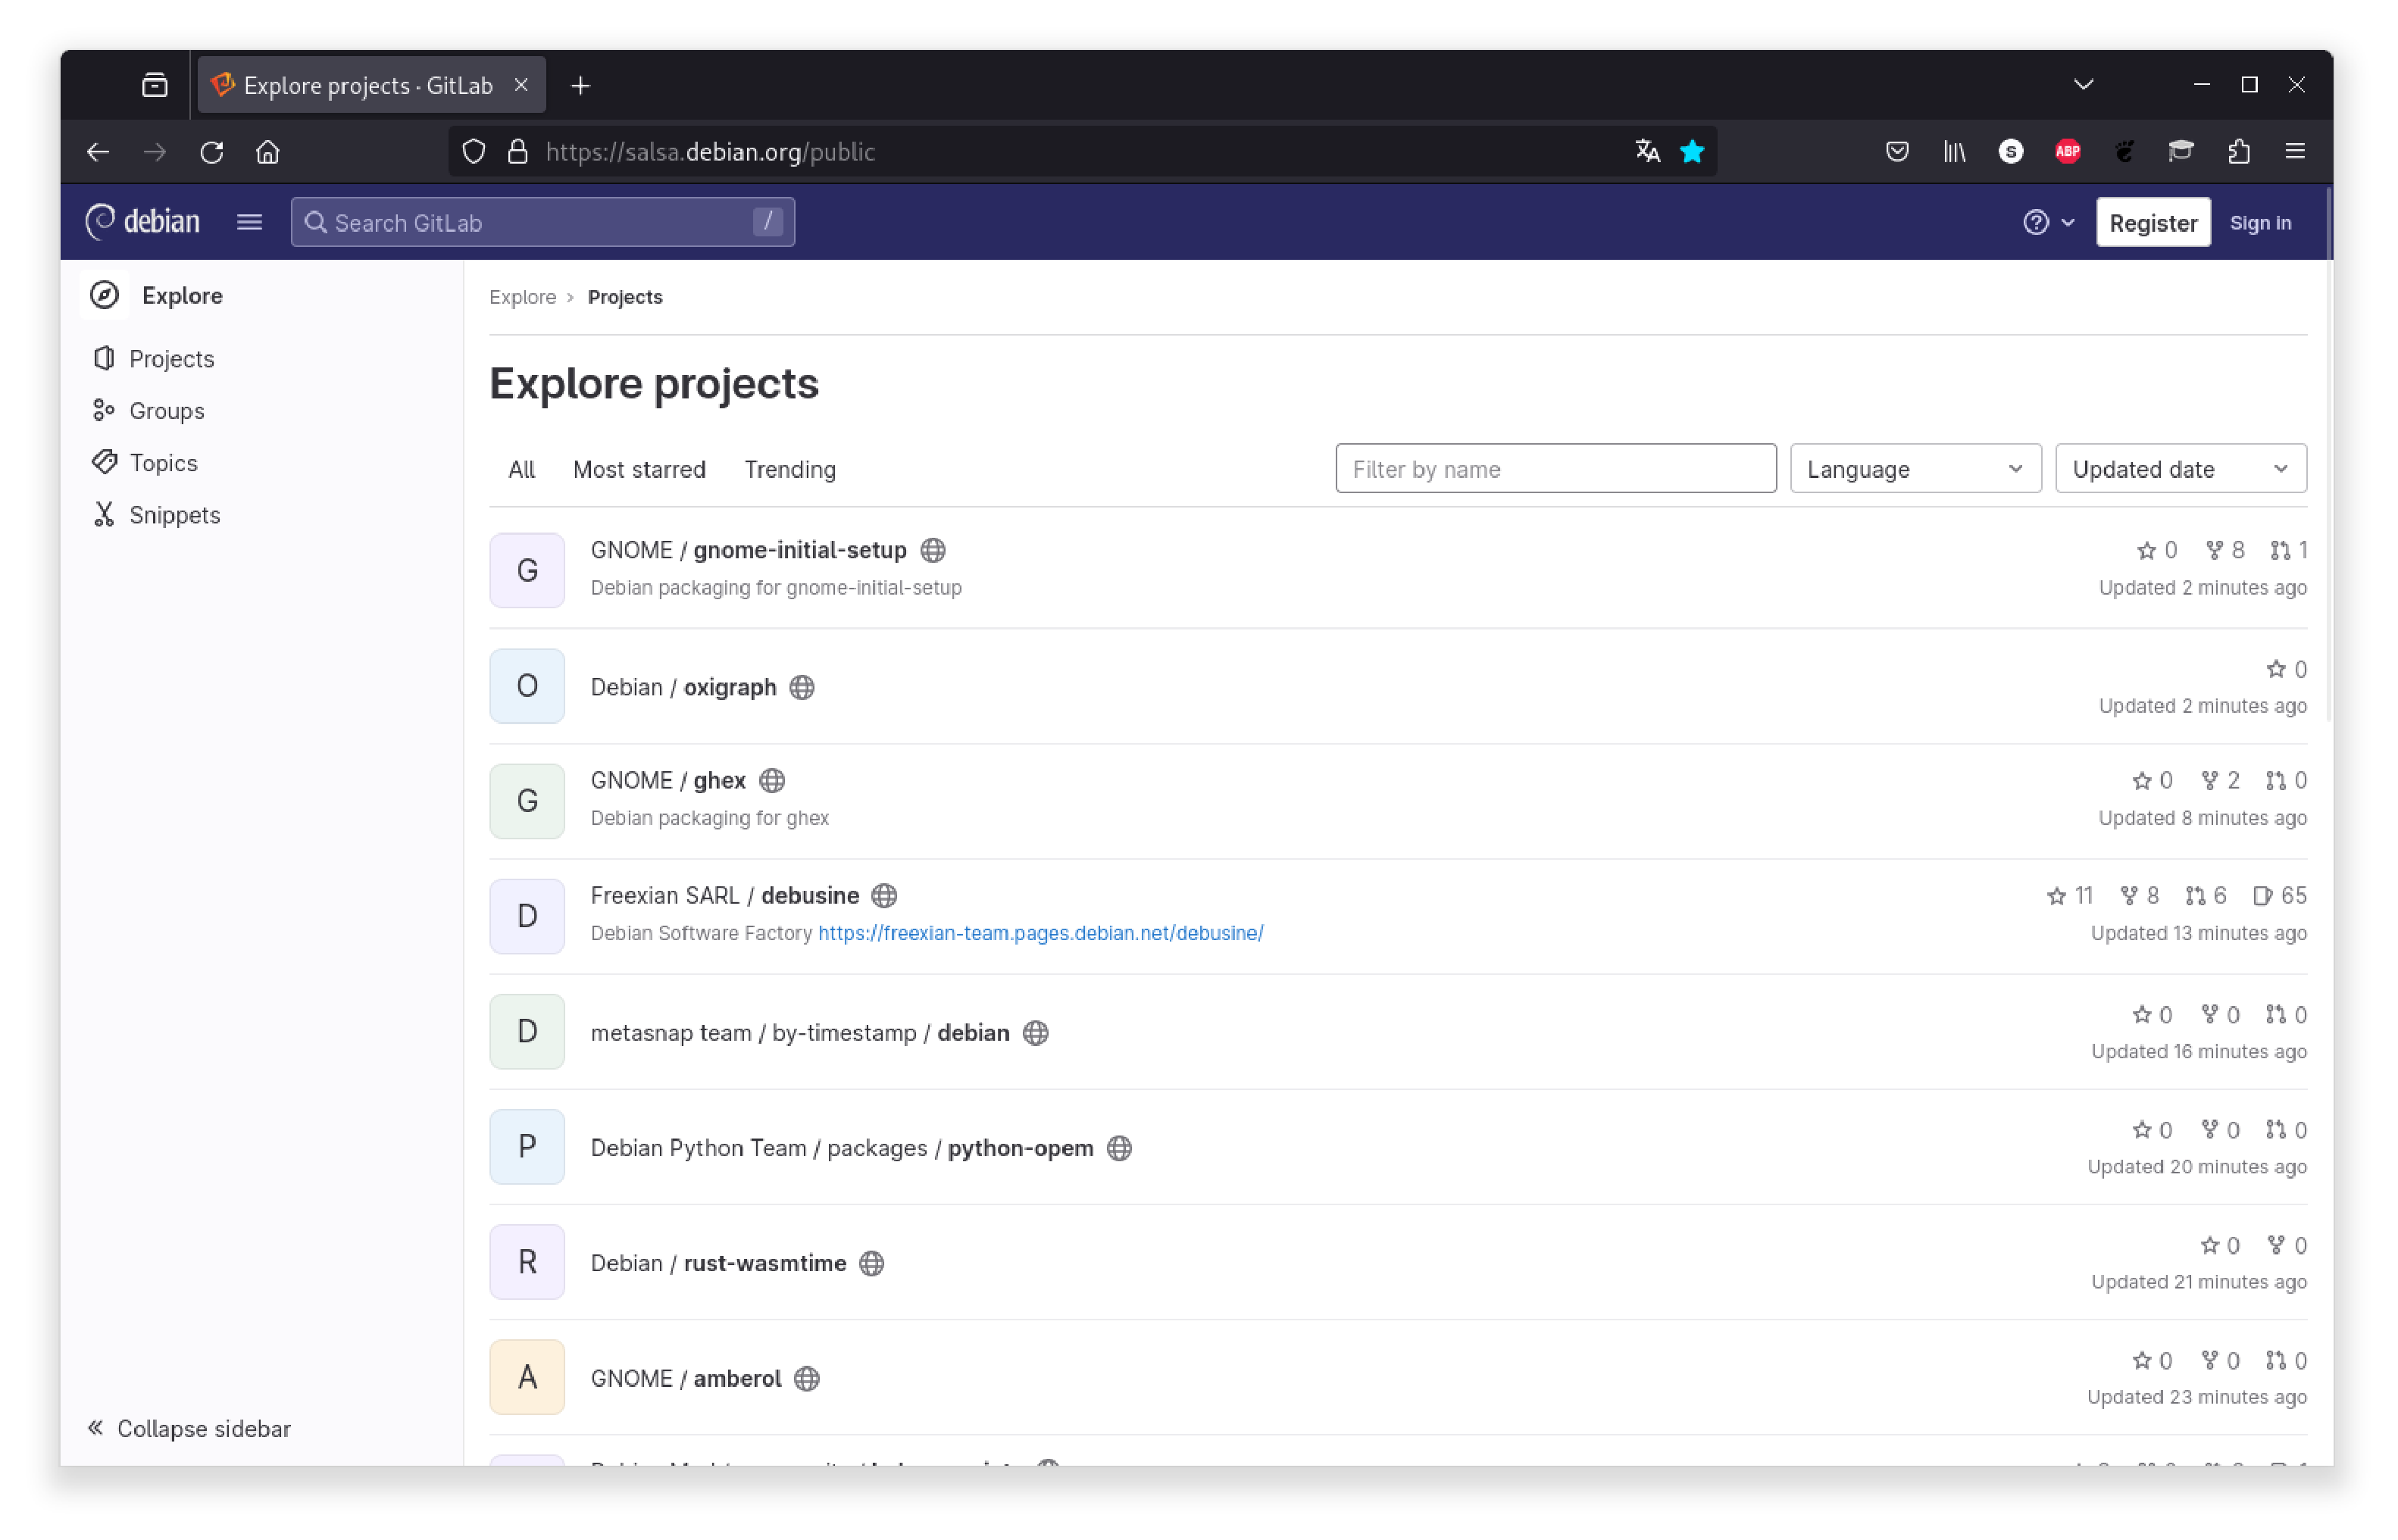
\includegraphics[width=1.0\textwidth,keepaspectratio=true,draft=\ddst]{img/deb/salsa}
\caption{The Debian \salsa\ web site}\label{salsa}
\end{figure}

\subsubsection{Search for suitable Debian packaging team}

In order to find a mentor and a sponsor to help you to get your package approved, search for suitable teams on \href{https://wiki.debian.org/Teams}{https://wiki.debian.org/Teams}. \\
In particular browse the parts dedicated to:
\begin{itemize}
\item Blends teams: \href{https://wiki.debian.org/Teams\#Blends\_teams}{https://wiki.debian.org/Teams\#Blends\_teams}
\item Packaging teams: \href{https://wiki.debian.org/Teams\#Packaging\_teams}{https://wiki.debian.org/Teams\#Packaging\_teams}
\end{itemize}
This is where you are likely to get in touch with people interested by your software. \\
For example to package "\href{https://atomes.ipcms.fr}{\bf{atomes}}" I got in touch with the \href{https://wiki.debian.org/Debichem}{Debichem} team. 

\newpage

\subsubsection{Post an ITP message that will appear on WNPP}

\href{http://www.debian.org/devel/wnpp/}{WNPP} Debian Official Work-Needing and Prospective Packages, is the official Debian website that holds, 
among other things, the list of the prospective packages for the Debian community: 
\begin{itemize}
\item Packages being worked on ({\bf{I}}ntent {\bf{T}}o {\bf{P}}ackage)
\item Requested packages ({\bf{R}}equest {\bf{F}}or {\bf{P}}ackaging)
\end{itemize}
By posting an ITP message on Debian's WNPP you are announcing that you intend to do the packaging yourself. 
If your package meets Debian standards, then you can look for a Mentor and Sponsor to review your package and upload it. \\[0.25cm]
To post the ITP message requires to use the command line and the \href{https://wiki.debian.org/reportbug}{"\texttt{reportbug}"} utility:
\begin{enumerate}
\item Prepare a complete text message that describe your package, including:
\begin{itemize}
\item Short description
\item Long description
\item Demonstration of the interest for the community
\item Request for sponsorship
\end{itemize}
A detailed example is provided in appendix \ref{bugreport}. 
\item Configure "\texttt{reportbug}":
\begin{enumerate}
\item Run "\texttt{reportbug --configure}" to create a "\texttt{\textasciitilde/.reportbugrc}" configuration file.
\item Follow the instructions and when asked: \\
"\texttt{Do you have a 'mail transport agent' (MTA) ... configured ?}" \\
choose \bftt{No}
\item Then enter the SMTP host for your mail server
\item For the user name enter your email address
\item For the question: \\
"\texttt{Does your SMTP host require TLS authentication ?}" \\
choose \bftt{Yes}
\end{enumerate}
You can edit the file "\texttt{\textasciitilde/.reportbugrc}" in particular to add your password:
{\footnotesize{
\begin{scriptii}
\uprompt{~} vi .reportbugrc
\comm{ reportbug preferences file}
\comm{ character encoding: UTF-8}
\comm{ Version of reportbug this preferences file was written by}
reportbug\_version \rtt{"7.10.3+deb11u1"}
\comm{ default operating mode: one of: novice, standard, advanced, expert}
mode novice
\comm{ default user interface}
ui text
\comm{ offline disables querying information over the network}
\comm{offline}
\comm{ name and email setting (if non-default)}
realname \rtt{"Your Name"}
email \rtt{"\email"}
\comm{ Send all outgoing mail via the following host}
smtphost \rtt{"www.webserver.eu"}
smtpuser \rtt{"\email"}
smtppasswd \rtt{"Your-Password-Here"}
\comm{ Require STARTTLS for the SMTP host connection}
smtptls
\comm{ If nothing else works, remove the \# at the beginning}
\comm{ of the following three lines:}
\comm{no-cc}
\comm{list-cc-me}
\comm{smtphost reportbug.debian.org}
\comm{ You can add other settings after this line.  See}
\comm{ /etc/reportbug.conf for a full listing of options.}
\end{scriptii}
}}
\item Use "\bftt{reportbug} \rtt{wnpp}" to send your ITP message:
{\footnotesize{
\begin{scripti}
\uprompt{~} \bftt{reportbug} \rtt{wnpp}
\end{scripti}
}}
\\[-0.75cm]
\noindent Then simply follow the prompt: 
\begin{enumerate}
\item This is an ITP
\item Enter the proposed package name: "\texttt{program}"
\item Enter the short description 
\item Press "\texttt{s}" to skip he bug message search
\item Complete and send the message, note that "\texttt{reportbug}" uses a \href{https://www.vim.org}{vi} interface:
\begin{itemize}
\item To insert text press \keystroke{i}, then input your text. \\
To navigate the document use the keyboard arrows \LArrow, \RArrow, \UArrow and \DArrow.
\item To save the message and to send it:
\begin{itemize}
\item Press \Esc
\item Press \keystroke{:}
\item Input: \\[-1cm]
\begin{scriptiii}
\texttt{x!}
\end{scriptiii}
\\[-1.5cm]
\item Press \Enter
\end{itemize}
\end{itemize}
Note that you can modify each line from the "\texttt{Subject}" first line to end of the message, 
including the package name and the short description if required.
\end{enumerate}
\end{enumerate}
When the message has been sent you will receive an email carbon copy of your message, as well as another message acknowledging your request and including a bug number as well as a link to follow the discussion on-line. \\
This message will have the following subject: 
\begin{script}
Bug#\rtt{???????}: Acknowledgment (\magenta{ITP:} \bftt{program} \magenta{--} \bftt{short description})
\end{script}
\\[-0.75cm]
\noindent where "\rtt{???????}" is the bug number associated with your ITP. \\
The link to follow the discussion on-line will be like:
\begin{script}
https://bugs.debian.org/cgi-bin/bugreport.cgi?bug=\rtt{???????}
\end{script}
\\[-0.75cm]
Now what's left is to introduce your self to the Debian packaging community. 

\subsubsection{Introduce yourself to the Debian community}

Simply send an email to the team you identify in the previous stage, to introduce your self, your work, and of course your program, also do not forget to mention the ITP bug number on WNPP. \\
Remember that Debian puts a lot of focus on quality, thus the better your package is prepared before submitting the ITP the easier it will be to find sponsorship. Sponsors might be hard to find and busy, helping them out to do the job is helping your package to be accepted more easily. \\
You can always get help from:
\begin{itemize}
\item Other members of a packaging team: \href{https://wiki.debian.org/Teams}{https://wiki.debian.org/Teams}
\item The Debian Mentors group (if your package does not fit in a team):
\begin{itemize}
\item \href{https://wiki.debian.org/DebianMentorsFaq}{https://wiki.debian.org/DebianMentorsFaq}
\item \href{http://mentors.debian.net/}{http://mentors.debian.net/}
\item The mentors mailing list: \href{mailto:debian-mentors@lists.debian.org}{debian-mentors@lists.debian.org}
\end{itemize}
\item Documentation: \href{http://mentors.debian.net/intro-maintainers}{http://mentors.debian.net/intro-maintainers}
\item Localized mailing list (in your own language) "debian-devel-\{language\}@lists.d.o":
\begin{itemize}
\item \href{mailto:debian-devel-french@lists.d.o}{debian-devel-french@lists.d.o}
\item \href{mailto:debian-devel-spanish@lists.d.o}{debian-devel-spanish@lists.d.o}
\end{itemize}
\end{itemize}

\subsubsection{After that: the next steps}

As for the RPM side, the next steps of the process are not up to you, or not entirely anyway.
As soon as both personal introduction and bug message have been sent, the community feedback
is required for your package to go further. 
Debian Mentors and Packager(s) will look into your bug message to test your package. 
The more your ensured that your package follows the official Debian packaging guidelines
the more easily your package will be accepted.
The most complicated part is likely to find a Mentor, an official Debian package maintainer
experienced enough to be allowed to register new package and their maintainer. This is done
via exchanges with the Debian packaging community, here are some advise:
\begin{itemize}
\item The process can take time: be patient !
\item Search for people that could be interested by your software in the community: remember
that a good introduction is the best starting point !
\item When you have someone to talk to, ask what to do to help: be part of the process all the
way through !
\end{itemize}

\subsection{Managing your official DEB package for Debian}

At this point I will assume that your DEB package has been approved by your mentor. \\
When done she or he, will create the official repository on \salsa. \\ 
Togheter you will have decided on the most suitable packaging team for your program. \\ 
Each teams has a group on \salsa, for example the Debichem team  
regroups chemistry related packages: \href{https://salsa.debian.org/debichem-team}{https://salsa.debian.org/debichem-team}. \\[0.25cm]
You can search for teams and the corresponding group on \salsa\ at: \\[0.25cm]
\href{https://wiki.debian.org/Teams\#Packaging\_teams}{https://wiki.debian.org/Teams\#Packaging\_teams} \\[0.25cm]
Then "Request Access" to the packaging team for your package. \\[0.25cm]
Your mentor will create a repository for your package in the selected packaging team, once the membership granted you will be able 
to upload data in your repository on \salsa\ at the address: \\[0.25cm] 
https://salsa.debian.org/PACKAGING-team/Program \\[0.25cm]
The official respository for your package on \salsa\ will contain 3 branches:
\begin{itemize}
\item "\texttt{upstream}": the sources of your program
\item "\texttt{pristine-tar}": the "\texttt{orig}" archive for your package, that contains both sources and the "\texttt{debian}" directory to build the DEB package. 
\item "\texttt{master}": the sources of your program and the "\texttt{debian}" directory to build the DEB package
\end{itemize}

\newpage
